\documentclass{article}\usepackage[]{graphicx}\usepackage[]{color}
% maxwidth is the original width if it is less than linewidth
% otherwise use linewidth (to make sure the graphics do not exceed the margin)
\makeatletter
\def\maxwidth{ %
  \ifdim\Gin@nat@width>\linewidth
    \linewidth
  \else
    \Gin@nat@width
  \fi
}
\makeatother

\definecolor{fgcolor}{rgb}{0.345, 0.345, 0.345}
\newcommand{\hlnum}[1]{\textcolor[rgb]{0.686,0.059,0.569}{#1}}%
\newcommand{\hlstr}[1]{\textcolor[rgb]{0.192,0.494,0.8}{#1}}%
\newcommand{\hlcom}[1]{\textcolor[rgb]{0.678,0.584,0.686}{\textit{#1}}}%
\newcommand{\hlopt}[1]{\textcolor[rgb]{0,0,0}{#1}}%
\newcommand{\hlstd}[1]{\textcolor[rgb]{0.345,0.345,0.345}{#1}}%
\newcommand{\hlkwa}[1]{\textcolor[rgb]{0.161,0.373,0.58}{\textbf{#1}}}%
\newcommand{\hlkwb}[1]{\textcolor[rgb]{0.69,0.353,0.396}{#1}}%
\newcommand{\hlkwc}[1]{\textcolor[rgb]{0.333,0.667,0.333}{#1}}%
\newcommand{\hlkwd}[1]{\textcolor[rgb]{0.737,0.353,0.396}{\textbf{#1}}}%
\let\hlipl\hlkwb

\usepackage{framed}
\makeatletter
\newenvironment{kframe}{%
 \def\at@end@of@kframe{}%
 \ifinner\ifhmode%
  \def\at@end@of@kframe{\end{minipage}}%
  \begin{minipage}{\columnwidth}%
 \fi\fi%
 \def\FrameCommand##1{\hskip\@totalleftmargin \hskip-\fboxsep
 \colorbox{shadecolor}{##1}\hskip-\fboxsep
     % There is no \\@totalrightmargin, so:
     \hskip-\linewidth \hskip-\@totalleftmargin \hskip\columnwidth}%
 \MakeFramed {\advance\hsize-\width
   \@totalleftmargin\z@ \linewidth\hsize
   \@setminipage}}%
 {\par\unskip\endMakeFramed%
 \at@end@of@kframe}
\makeatother

\definecolor{shadecolor}{rgb}{.97, .97, .97}
\definecolor{messagecolor}{rgb}{0, 0, 0}
\definecolor{warningcolor}{rgb}{1, 0, 1}
\definecolor{errorcolor}{rgb}{1, 0, 0}
\newenvironment{knitrout}{}{} % an empty environment to be redefined in TeX

\usepackage{alltt}
\usepackage[top=1.00in, bottom=1.0in, left=1.00in, right=1.00in]{geometry}
\renewcommand{\baselinestretch}{1.1}
\usepackage{graphicx}
\usepackage{float}
\usepackage{natbib}
\usepackage{amsmath}
\bibliographystyle{..//refs/styles/besjournals.bst}
\parindent=24pt
\def\labelitemi{--}
\usepackage{lineno}

\usepackage{xr-hyper}
\externaldocument{FLSshort_supp}
\IfFileExists{upquote.sty}{\usepackage{upquote}}{}
\begin{document}
\section*{plan 1}
Background note: 162 pots can fit in each (2) growth chambers and get direct light. More can fit in chillin chambers on shelves.\\
Due to these space limitations, I propose doing applying in the chambers and forcing in the greenhouse since the focus for this study is not about the specifics of the temperature response (will discuss more below).

9pots [response surface] * 3 [species] * 2 [chill] * 2 [nutrients] * 2 [harvest dates] = 648 pots or\\
9pots [response surface] * 3 [species] * 3 [chill] * 2 [nutrients] * 2 [harvest dates] = 972 pots.

\subsection{Response surface}
Because of varaibility in germination, I don't want to have too low densities that it is possible that no seeds germinate. 9 pots per RS is idea for spacing in chambers. Two total densities of 8 max per pot and 16. (Could also do 4)

\begin{knitrout}
\definecolor{shadecolor}{rgb}{0.969, 0.969, 0.969}\color{fgcolor}
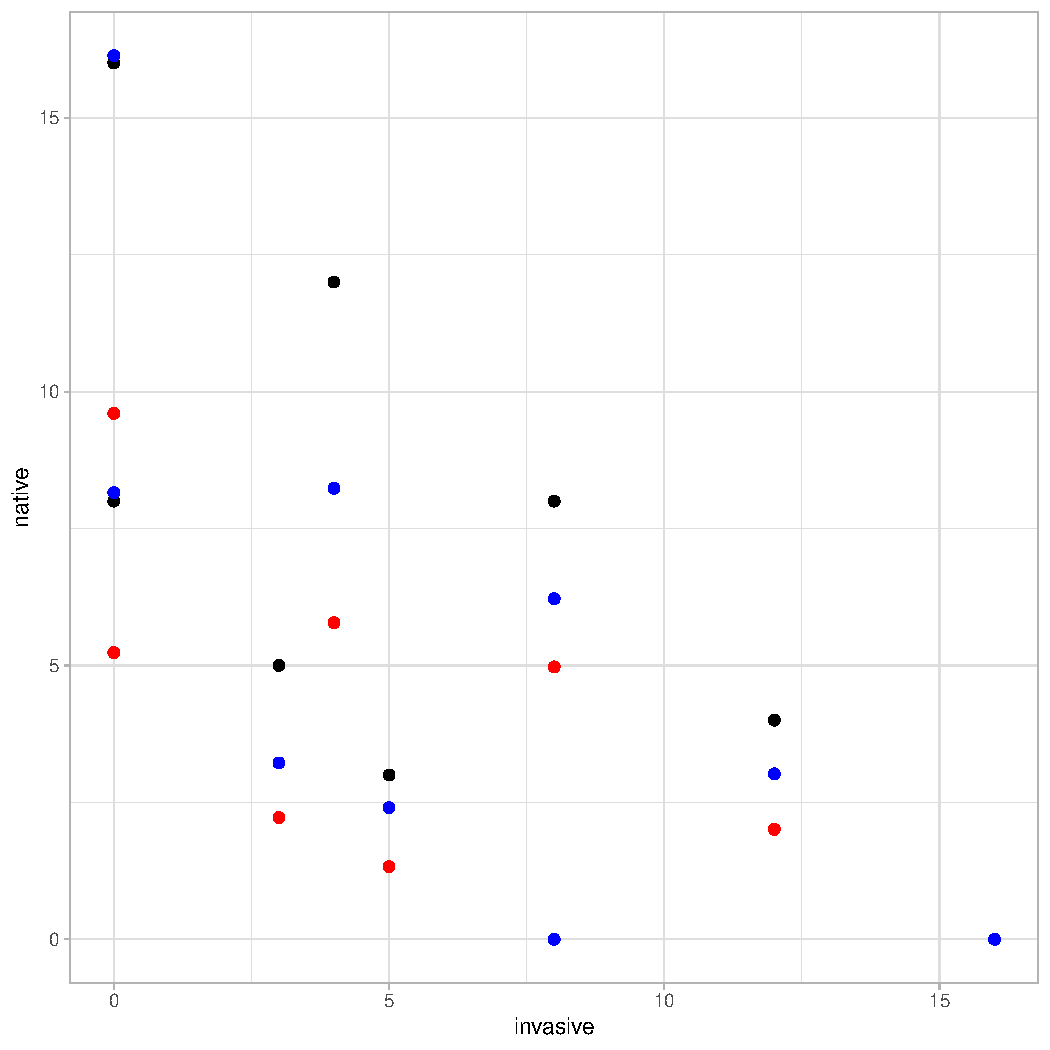
\includegraphics[width=\maxwidth]{figure/unnamed-chunk-1-1} 

\end{knitrout}

\subsection{species and climate treatment}
\textit{H. matronalis}, \textit{P. virginiatum}, \textit{C. canadensis}.\\

 \begin{figure}[h!]
        \centering
          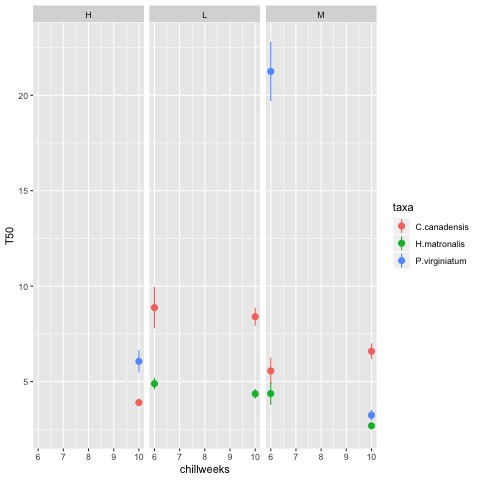
\includegraphics[width=\textwidth]{prelimT50.jpeg}

    \end{figure}    

As we can see, most of the action happens at M forcing (20/10) and chilling has a much stronger effect on T50. (Unfortunately I didn't test the Polygonum at low temperatures, but I do not think it would have germinated reasonably based at low chilling).

\subsection{Nutrients}
Nutrient availability might interact with the importance of the priority effect. Also, after 1 month in the greenhouse, all plants seem nutrient deficient (P and N). Challange: If some plants germinated early and other late, applying nutrients might shock those still in the cotyledon phase.\\
Proposal to run by Lee:\\
\textbf{High nutrient:} Layer of fertilizer at bottom of pot long roots could reach eventually. Plus weekly fertilizer application after germination window.\\
\textbf{Low nutrient:} Monthly fertilizer application after germination window\\.

\subsection{Multiple Harvests}
We don't want to conflate final biomass estimates with ontonogy. ie if we harvest now (after 1 month), many later germinators are still cotyledons. Harvest 2 crops, eg one after 1 month and 1 after 3 months ensures some data, and shows how the priority effects might change over time.\\
\textbf{Harvest 1:} 7 weeks after transfer to focing conditions (3 weeks for germination and 4 for growth).\\
\textbf{Harvest 2:} 15 weeks after transfer to focing conditions (3 weeks for germination and 12 for growth).\\

\subsection{Other considerations:}
\begin{itemize}
\item Is the grid neccisary or is it better to mix seeds and randomly sow them now that I can identify species based on cotyledon.
\item How to account for differences in sowing density vs final density: ie 100\% germination of Dames rocket and 60\% germination of other.
\begin{itemize}
\item We are already accounting for density effects, and this might be a strength because we could test for differences between sowed and realized densities as a function of germination speed of competitor. Would specify whether competion is acting on the seed or seedling.
\end{itemize}
\item Order new seeds or use ones that have been stored in fridge at 2.5\degree C?
\item Does it matter if I a) pot up all at once and start chilling together with subsequent removal vs. stagger start of chilling (long first, short second etc) and trasfer to forcing all at once to minimize the total duration of time I am making daily observations?
\item Should I go through the trouble of biomassing the pilot study?
\end{itemize}
\end{document}
